\documentclass[12pt,a4paper,final]{report}			%definire grandezza testo, foglio e tipo di testo.

\usepackage[svgnames]{xcolor} % Required for colour specification

%				** TIPI DI DOCUMENTI **
%			- article
%			- book
%			- report
%			
%
\usepackage[utf8]{inputenc}			%definisce la codifica dei caratteri
\usepackage[english]{babel}				%definisce il pacchetto della lingua
\usepackage{amsmath}						%contiene molti utili strumenti per la scrittura matematica
\usepackage{amsfonts}
\usepackage{amssymb}
\usepackage{makeidx}
\usepackage{graphicx}
\usepackage{lmodern}
\usepackage{units}  					%unita di misura
\usepackage{pgfplots}				%grafici
\usepackage{subcaption}  		%per le figure
\usepackage{gensymb} 			%per i gradi
\usepackage{pst-solides3d}  %per figure in 3D
%\usepackage{hyperref}				%permette di linkare
\usepackage{circuitikz}			%per circuiti
\usepackage{pgfplots}				%per fare plot pgf
\usepackage{subcaption}		%DON'T KNOW. INVESTIGATE
\usepackage{siunitx} 				%unita SI
\usepackage{wrapfig}				%per mettere più immagini insieme
\usepackage{bbold}					%per avere numeri in \mathbb{}
\usepackage{mathrsfs}			%per usare cose tipo \mathscr{}
\usepackage{physics}				%contiene molta notazione utile; lo uso in particolare per \bra e \ket
\usepackage{pgfplotstable}	%DON'T KNOW. INVESTIGATE
\usepackage{titlesec}				%per formattare titoli, paragrafi etc.
\usepackage{xfrac}
\usepackage{cite}
\usepackage{caption}
\usepackage[font=small,labelfont=bf]{caption}		% serve per ridurre la dimensione delle captions
\usepackage[final]{pdfpages}		%per poter includere pdf

\usepackage[a-1b]{pdfx}
\usepackage[pdfa]{hyperref}

\title{Thesis Summary}

\begin{document}
\begin{center}
	\Huge 
	Thesis Summary
\end{center}
\medskip 
%	In my thesis I have analyzed and classified the signature of cosmic rays in the timelines measured by Planck/HFI data using Convolutional Neural Networks (CNNs).	
		
	The \textbf{Standard Model of Cosmology} predicts that the present Universe began some 14 billion years ago through a mathematical singularity, the Big Bang, and started expanding. Matter and radiation were, at the beginning, a hot plasma in thermal equilibrium. Due to the expansion, this primordial plasma gradually cooled down and, after around $380,000~\unit{yr}$, it was cold enough for atoms to form.  
	The sharp decrease in the cross section of Thomson scattering permitted the free propagation of photons. 
	To date, many experiments have been able to measure these primordial photons, also known as \textbf{Cosmic Microwave Background} (CMB). 
	
	The space mission \textbf{Planck}, by the \textit{European Space Agency}, has given to date some of the most accurate measurements of CMB anisotropies, differences in temperature of the photons across the sky. 
	Planck implemented two instruments, which probed the sky in two different frequency ranges: \textbf{LFI} covered the $30–70~\unit{GHz}$ range, and \textbf{HFI} the $100–850~\unit{GHz}$ range. 
	LFI, \textit{low frequency instrument}, used radiometers kept at $20~\unit{K}$.
	HFI, \textit{high frequency instrument}, consisted of $48$ bolometers, nearly perfect absorbers kept at $0.1~\unit{K}$  and connected to solid state thermometers that measure changes in temperature of the absorber itself.
	
	While both instruments were prone to systematics due to \textbf{cosmic ray }hits, this was particularly true for HFI.
	When cosmic rays managed to reach HFI bolometers, they induced a signature in the temperatures acquired by the thermometers. These signatures are labeled as \textbf{glitches}. 
	The Planck/HFI collaboration already managed to remove these glitches from the raw data using an algorithm based on the \textit{rms} measured in the timelines. 
	
	The target of my thesis is to analyze and classify the signature of cosmic rays in the timelines using an alternative approach, based on \textbf{Convolutional Neural Networks}.
%		In my thesis I have analyzed and classified the signature of cosmic rays in the timelines measured by Planck/HFI data using Convolutional Neural Networks (CNNs).
	
	A \textbf{Neural Network} is made of a set of \textit{layers}, and produces an output starting from some input, in a deterministic way. The network computes the output by means of numbers, called \textit{weights}, associated to each layer. The values of the \textit{weights} are set through a process called \textbf{learning}.
	Some \textbf{training data}, which is classified by hand, is given to the network, which produces the output. In order to learn, the output is compared to the expected result, and a \textit{loss score} is computed. An \textit{optimizer} changes the weights to get a better score. The training is repeated many times, until some convergence criterion is reached. If the process is successful, the network will be able to produce sensible output from new unseen data, provided that its features are similar to that of the training data.
	
	I chose a \textbf{Convolutional Neural Network} because of the following advantageous feature: \textit{translational invariance}. This means that, when the network learns a pattern in one part of a timeline, it will be able to recognize it anywhere else. My CNN is a classification network, as its purpose is to classify its input (a timestream of temperatures) as \textit{glitches} or not.
	
%	The raw data from Planck/HFI needed some preparation before the classification procedure. Through the use of the \textit{Planck 2018 Sky Map} at $353~\unit{GHz}$ from the \textit{Planck Legacy Archive} (PLA), I removed from my data pool those points whose positions matched those of the \textit{Interstellar Medium}. 
%	I also subtracted the dipole effect generated from the motion of the Solar System with respect to the rest frame of the CMB. This phenomenon generated an oscillatory behaviour whose peak-to-peak amplitude in the data is $\sim 3~\unit{mK}$.
%	
%	After cleaning the data, I built a computer program that would enable a by-hand classification of the data. I took timelines of $100$ samples long and selected them either as \textit{glitch} or \textit{non-glitch}. 

%	For the training set of my network, I prepared $1600$ timelines. The preparation consisted on cleaning the data, e.g. removal of dipole effect caused by the motion of the Solar System, and classifying it, either as \textit{glitch} or \textit{non-glitch}. I also classified some other $400$ timeseries as \textit{validation}: 
	I personally prepared the test dataset manually, classifying $2000$ datastreams acquired by HFI during the first days of the Planck mission. Of these, $400$ were used as \textit{validation}: their purpose was to check the performance of the network on data not utilized in the training. 
	This method permits to detect \textit{overfitting}, a situation in which the network performs well on the training set but poorly on unseen data, because of an excessive specialization. 
	
	I built the \textbf{Convolutional Neural Network} using 6 layers. I optimized the structure of the CNN by training it multiple times on different configurations, until I found the one that maximized the accuracy. The final \textbf{accuracy} reached, both on the training set and the validation set, is $97.71\%$. In the image below (Fig. \ref{only_figure}) I show two timeseries classified correctly.
	
	At last, I classified $100$ timelines for testing the network on new data. To compare it with the approach followed by the Planck/HFI collaboration, I wrote a program that identifies the presence of a glitch using an \textit{rms} threshold. 
	This algorithm divides each timeline into 7 batches (number obtained through some optimization), it takes the highest \textit{rms} between the 7 divisions and compares it with a threshold. 
	To discriminate, I used the lowest of the values computed from timelines classified as \textit{glitches}. 
	On these new $100$ testing timestreams, the \textit{rms} program classified correctly $97$ of them, while the network managed to label all of them as I did.
%	  This program managed to guess correctly $97\%$ of the testing data, while the network labeled correctly all of these timelines.
	
	In conclusion, in this thesis I showed a different type of approach to glitch classification. My \textbf{Convolutional Neural Network} managed to achieve a result above $95\%$ on every instance it was deployed when recognizing \textit{glitches}, even if trained on a small sample of data. My work is important in the context of future CMB missions based on bolometers, like the JAXA \textbf{LiteBIRD }mission, adopted in May 2019 and scheduled for launch in 2027.
	
\begin{figure}[h!]
				\centering
				\begin{subfigure}[t]{0.8\textwidth}		
				\centering		
					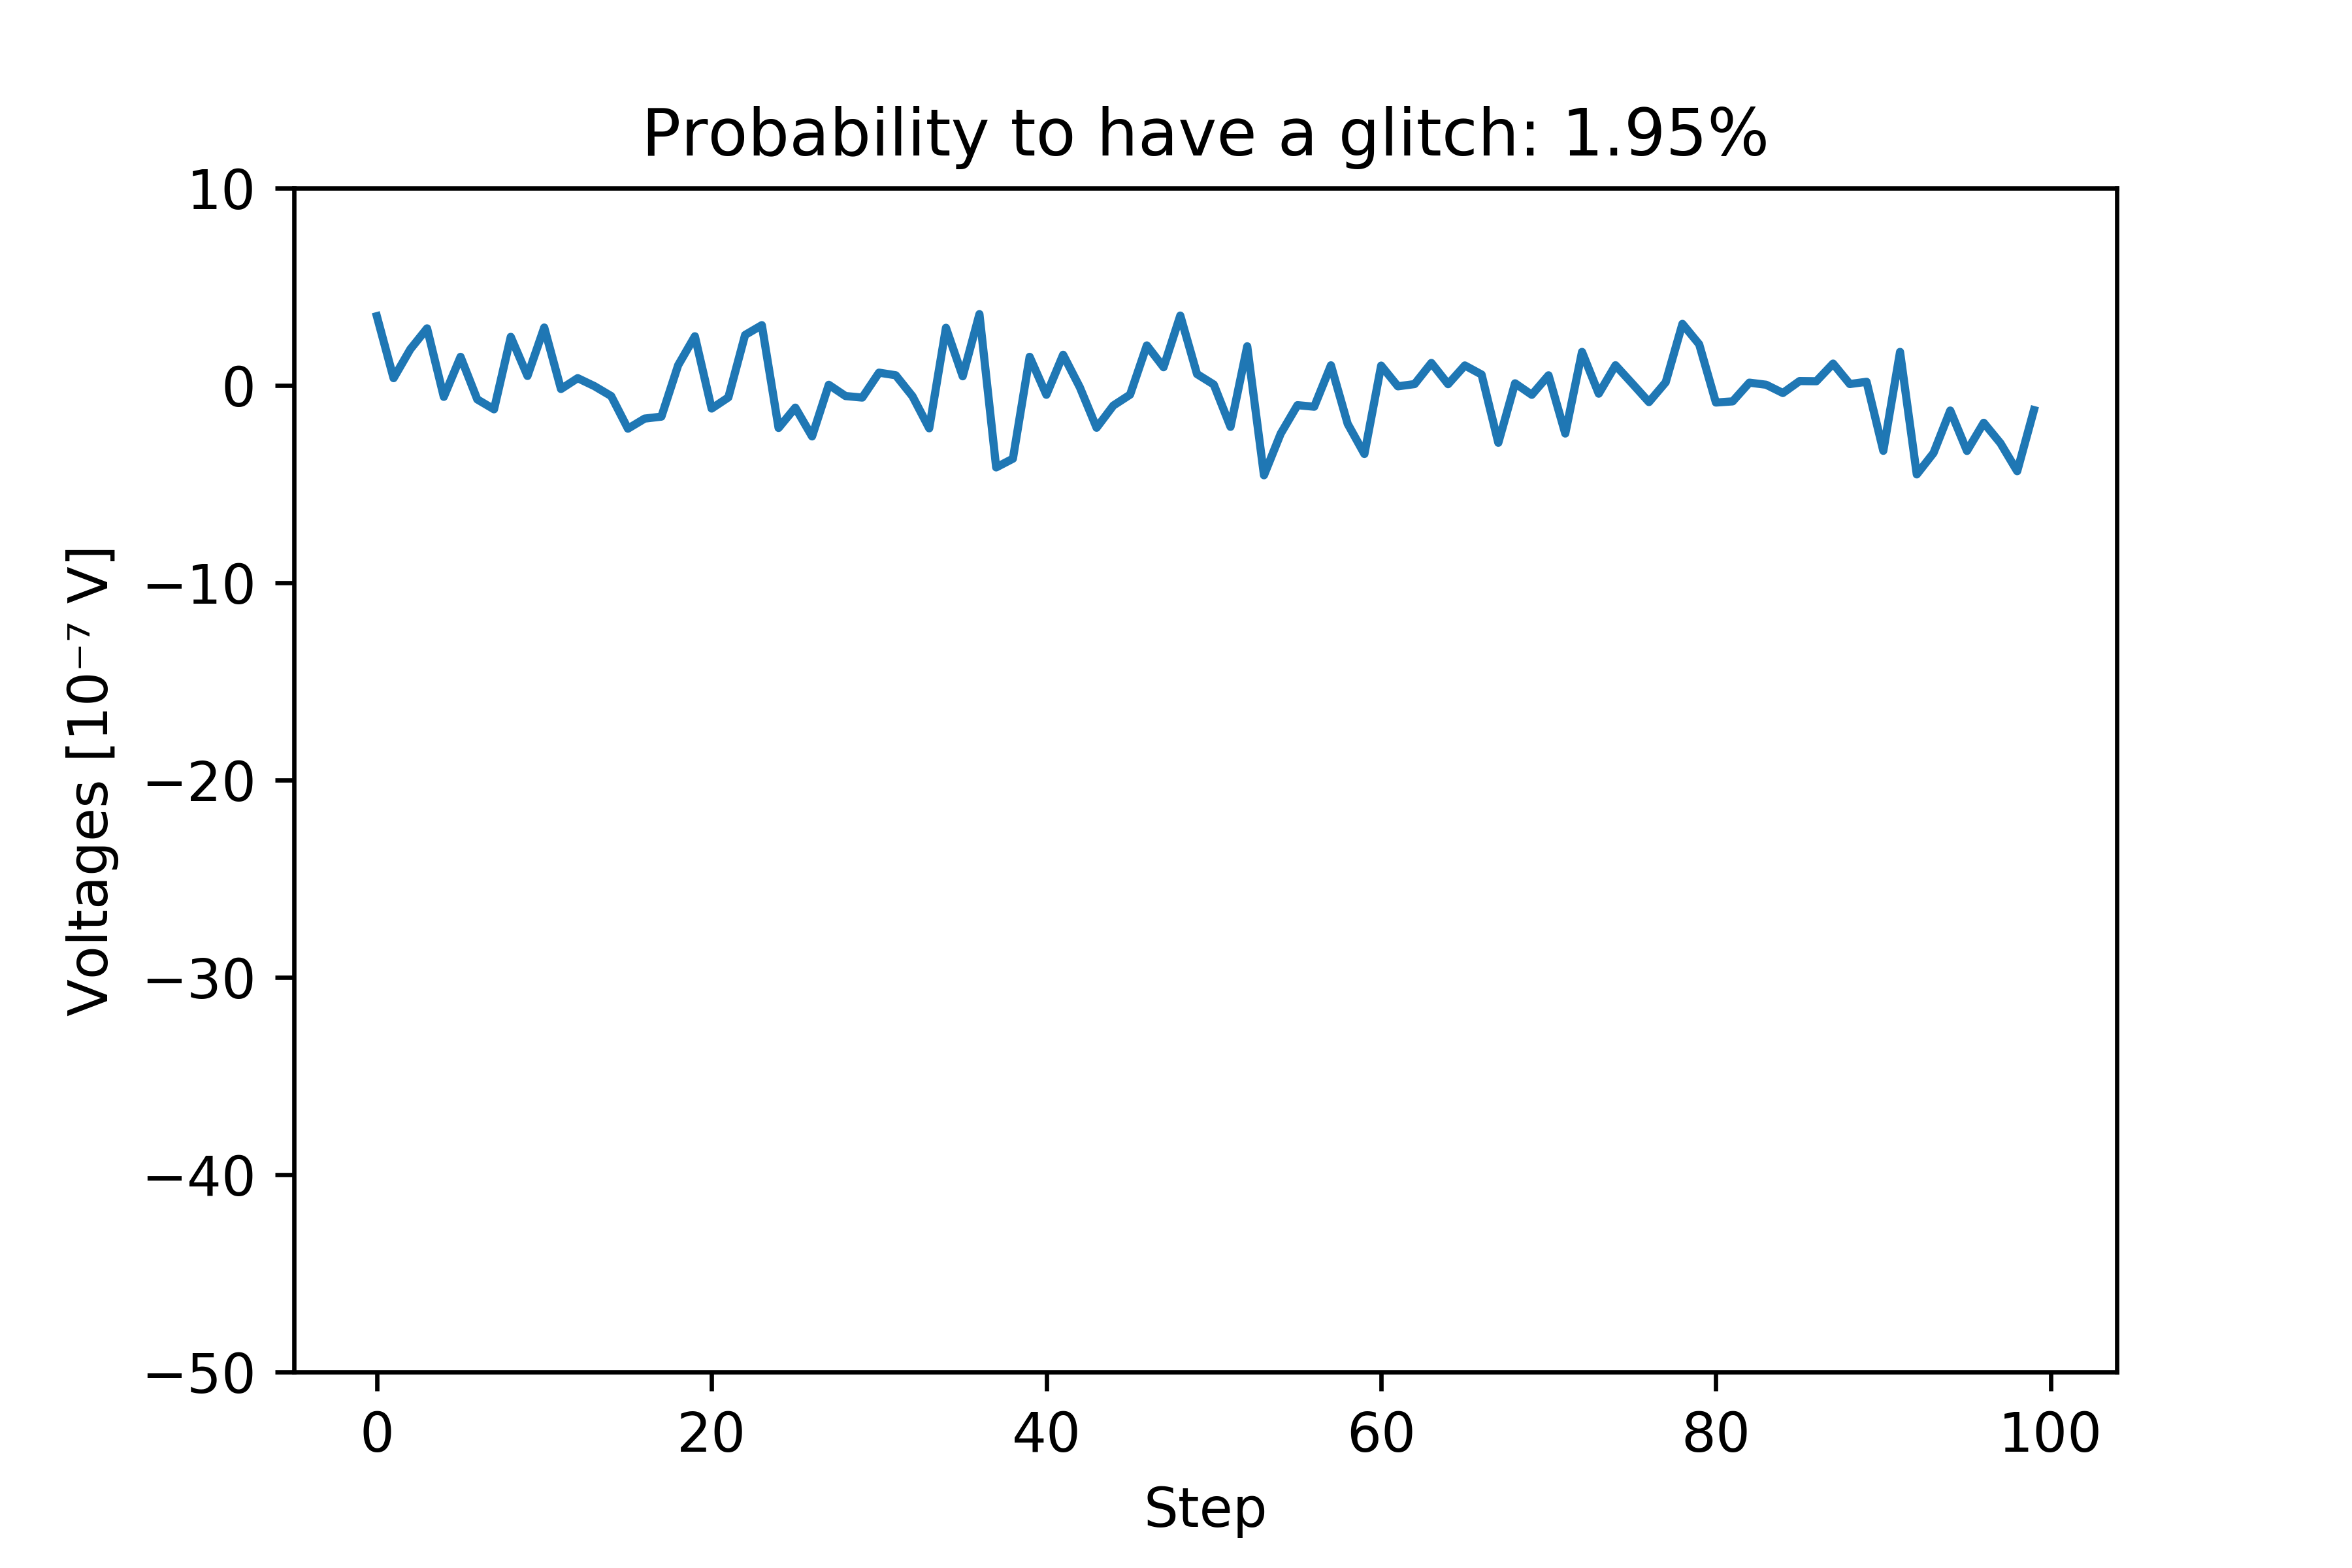
\includegraphics[scale=0.7]{../test_plots/plot_1.png}
				\end{subfigure}			

				\begin{subfigure}[t]{0.8\textwidth}				
				\centering
					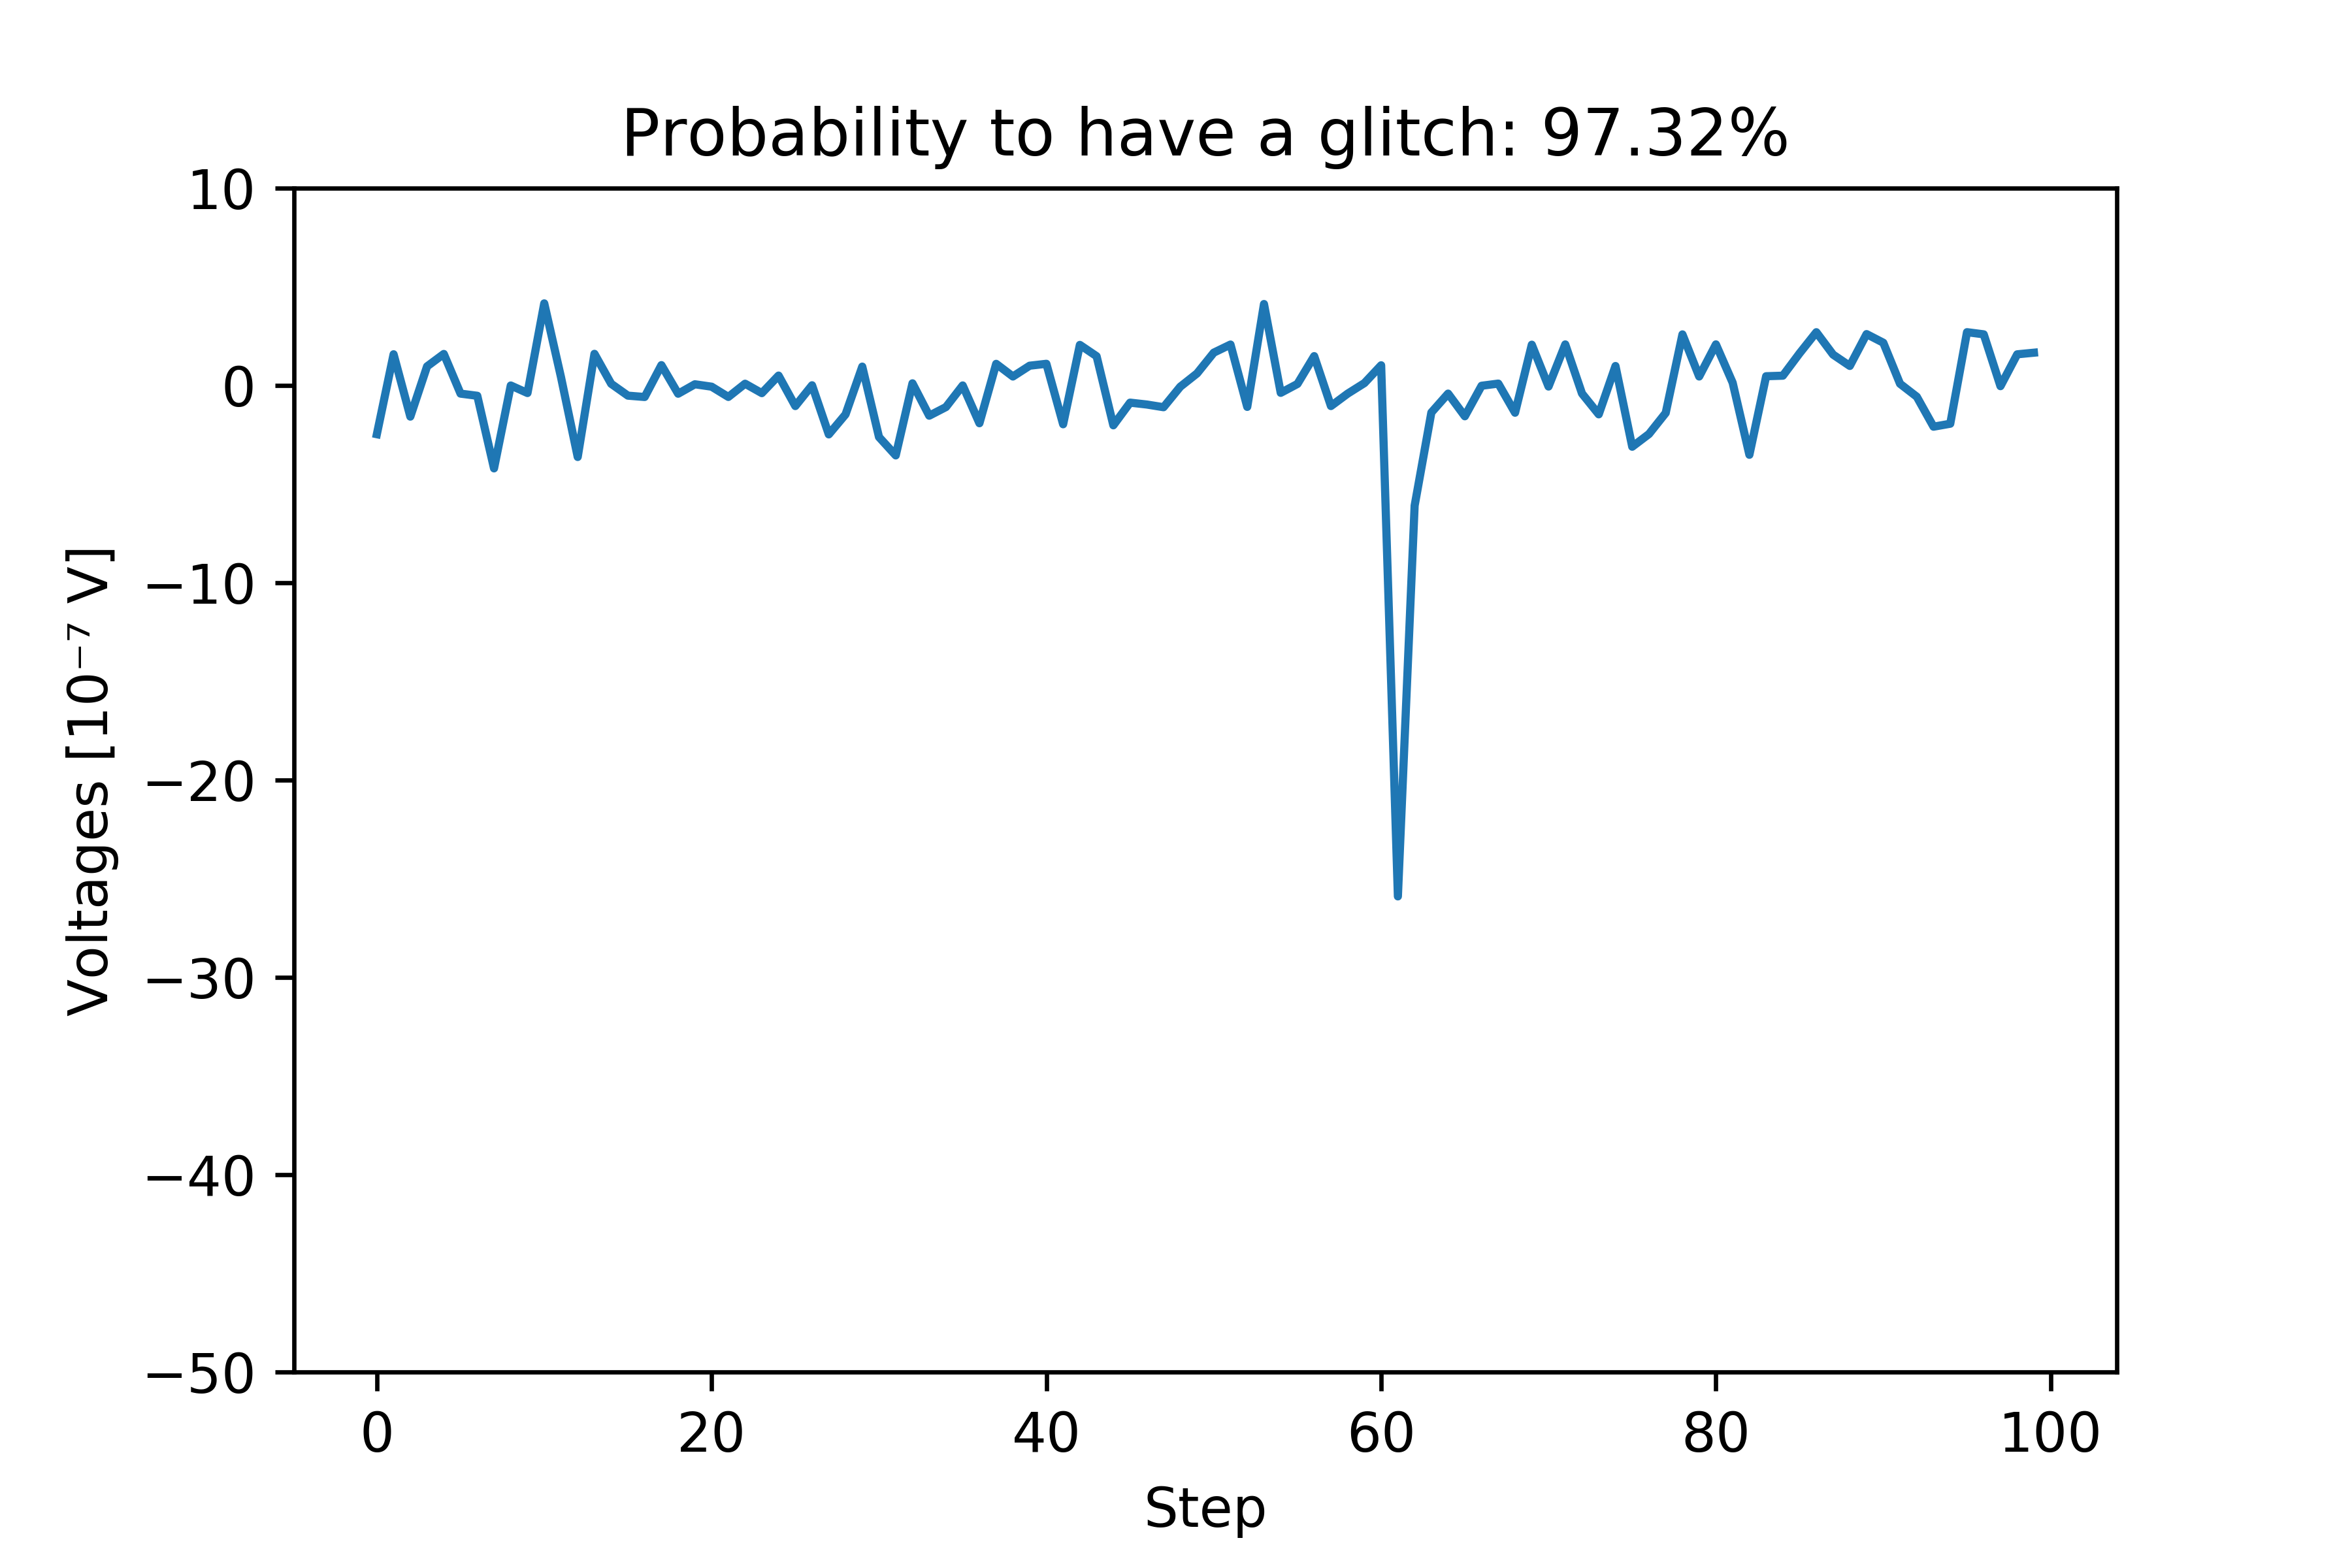
\includegraphics[scale=0.7]{../test_plots/plot_10.png}
				\end{subfigure}		
				\caption{}
				\label{only_figure}
				
	\end{figure}

\end{document}
